% !TEX TS-program = pdflatex
% !TeX program = pdflatex
% !TEX encoding = UTF-8
% !TEX spellcheck = fr

\documentclass[xcolor=table]{beamer}


%\usepackage{fullpage}
%\usepackage[left=2.8cm,right=2.2cm,top=2 cm,bottom=2 cm]{geometry}
\setbeamersize{text margin left=10pt,text margin right=10pt}
\usepackage{amsmath,amssymb} 
\usepackage[T1]{fontenc}
\usepackage[utf8]{inputenc}
\usepackage[english,french]{babel}
\usepackage{txfonts}
\usepackage[]{graphicx}
\usepackage{multirow}
\usepackage{hyperref}
\usepackage{colortbl}
\usepackage{listings}
\usepackage{wrapfig}
\usepackage{multicol}
\usepackage[export]{adjustbox} %for images in table, also for frame

\hypersetup{
	colorlinks,
	urlcolor = blue
}

%\renewcommand{\baselinestretch}{1.5}

\def\supit#1{\raisebox{0.8ex}{\small\it #1}\hspace{0.05em}}

\AtBeginSection{%
	\begin{frame}
		\sectionpage
	\end{frame}
}

\newcommand{\rottext}[2]{%
	\rotatebox{90}{%
	\begin{minipage}{#1}%
		\raggedleft#2%
	\end{minipage}%
	}%
}

\usepackage{longtable}
\usepackage{tabu}


\institute{ %
École  nationale Supérieure d'Informatique (ESI, ex. INI), Algérie
}
\author[ \textbf{\footnotesize  \insertframenumber/\inserttotalframenumber} \hspace*{\fill} ESI (2019-2020)] %
{ARIES Abdelkrime}
%\titlegraphic{
\includegraphics[height=1cm]{../img/esi-logo.png}%\hspace*{4.75cm}~


\date{Année unniversitaire: 2019/2020} %\today

\usetheme{Warsaw} % Antibes Boadilla Warsaw

\beamertemplatenavigationsymbolsempty

%\setbeamertemplate{headline}{}

\definecolor{lightblue}{HTML}{D0D2FF}
\definecolor{lightyellow}{HTML}{FFFFAA}
\definecolor{darkblue}{HTML}{0000BB}
\definecolor{olivegreen}{HTML}{006600}
\definecolor{violet}{HTML}{6600CC}

\newcommand{\keyword}[1]{\textcolor{red}{\bfseries\itshape #1}}
\newcommand{\expword}[1]{\textcolor{olivegreen}{#1}}
\newcommand{\optword}[1]{\textcolor{violet}{\bfseries #1}}

\makeatletter
\newcommand\mysphere{%
	\parbox[t]{10pt}{\raisebox{0.2pt}{\beamer@usesphere{item projected}{bigsphere}}}}
\makeatother

%\let\oldtabular\tabular
%\let\endoldtabular\endtabular
%\renewenvironment{tabular}{\rowcolors{2}{white}{lightblue}\oldtabular\rowcolor{blue}}{\endoldtabular}


\NoAutoSpacing %french autospacing after ":"

\def\graphpath{}

\newcommand{\changegraphpath}[1]{\def\graphpath{#1}}

\newcommand{\graphintable}[2]{%
	\includegraphics[height=#1,valign=t]{\graphpath #2}%
}

\newcommand{\vgraphpage}[2][.85\textheight]{%
	\begin{center}%
		\includegraphics[height=#1]{\graphpath #2}%
	\end{center}%
}

\newcommand{\hgraphpage}[2][\textwidth]{%
%	\begin{center}%
		\includegraphics[width=#1]{\graphpath #2}%
%	\end{center}%
}

\newcommand{\insertbibliography}[2]{
	\appendix
	\section*{Bibliographie}
	\nocite{#2}
	
	\begin{multicols*}{2}[\frametitle{\insertsection} \usebeamertemplate{frametitle}]%\usebeamertemplate*{frametitle}\frametitle{Références}
		\tiny
		\bibliography{#1}
		\bibliographystyle{acm}
	\end{multicols*}
}



\title[BWEB: 03- Rédaction] %
{Bureautique et Web \\Chapitre 03: Rédaction d'un document numérique\\ \slshape\small  Introduction}  

\changegraphpath{..//img/Bweb03-redaction/}

\begin{document}
	
	\newcolumntype{L}[2]{%
		>{\vbox to #2\bgroup\vfill\flushleft}%
		p{#1}%
		<{\egroup}} 

\begin{frame}[plain]
	\maketitle
\end{frame}

\begin{frame}
\frametitle{Rédaction d'un document numérique}
\framesubtitle{Introduction: Un peu d'humeur}

\vgraphpage{editing-humour.jpg}

\end{frame}

\begin{frame}
\frametitle{Rédaction d'un document numérique}
\framesubtitle{Introduction : Plan}

\begin{multicols}{2}
	%	\small
	\tableofcontents
\end{multicols}
\end{frame}

%===================================================================================
\section{Structure d'un rapport}
%===================================================================================

\begin{frame}
\frametitle{Structure d'un rapport}

\begin{itemize}
	\item pages préliminaires
	\begin{itemize}
		\item couverture
		\item remerciements
		\item résumé
		\item table des matières
		\item listes diverses (figures, tableaux, abréviations, symboles, algorithmes)
	\end{itemize}

	\item corps du texte
	\begin{itemize}
		\item introduction
		\item développement (chapitres)
		\item conclusion
	\end{itemize}

	\item pages complémentaires
	\begin{itemize}
		\item annexes et appendices
		\item glossaire
		\item index
		\item bibliographie
	\end{itemize}

\end{itemize}

\end{frame}

\subsection{Pages préliminaires}

\begin{frame}
\frametitle{Structure d'un rapport}
\framesubtitle{Pages préliminaires}

\begin{itemize}
	\item Pages qui précèdent le développement du rapport
	\item Toutes les pages sont numérotées, sauf la page de garde
	\item Les numéros de pages sont en chiffres romains (I, II, III, IV, V, etc.) 
\end{itemize}

\end{frame}


\begin{frame}
\frametitle{Structure d'un rapport: Pages préliminaires}
\framesubtitle{Couverture}

\begin{minipage}{0.52\textwidth}
	\begin{itemize}
		\item Nom de l'université 
		\item Année universitaire
		\item Sujet
		\item Nom de l'étudiant
		\item Nom de l'encadrant 
		\item Nom du laboratoire ou de l'entreprise
		\item Logos (université, entreprise, laboratoire)
	\end{itemize}
\end{minipage}
\begin{minipage}{0.42\textwidth}
	
\includegraphics[width=\textwidth]{..//img/Bweb03-redaction/couverture.png}
\end{minipage}

\end{frame}

\begin{frame}
\frametitle{Structure d'un rapport: Pages préliminaires}
\framesubtitle{Remerciements}

\begin{minipage}{0.52\textwidth}
	\begin{itemize}
		\item Promoteur (Organisme d'accueil)
		\item Encadreur (L'université)
		\item Personnes ayant contribué au travail (aide financière, révision, etc.) en mentionnant la nature de l'aide.
		\item Famille pour soutien
		\item ...
		\item Elles doivent être:
		\begin{itemize}
			\item \optword{simples}: pas d'exagération
			\item \optword{professionnelles}: moins de familiarité
		\end{itemize}
	\end{itemize}
\end{minipage}
\begin{minipage}{0.42\textwidth}
	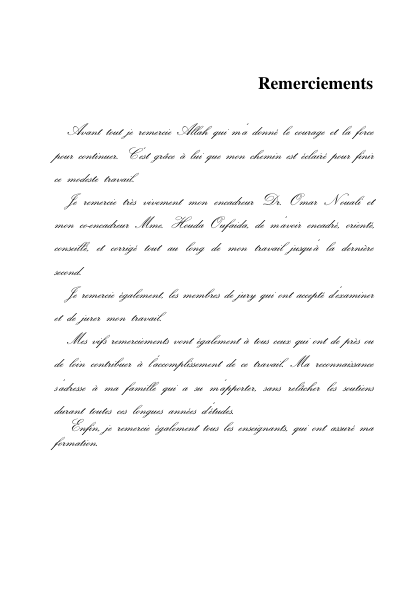
\includegraphics[width=\textwidth]{..//img/Bweb03-redaction/remerciements.png}
\end{minipage}

\end{frame}

\begin{frame}
\frametitle{Structure d'un rapport: Pages préliminaires}
\framesubtitle{Résumé}

\begin{minipage}{0.52\textwidth}
	\begin{itemize}
		\item Mini-version du rapport
		\item Il doit être:
		\begin{itemize}
			\item \optword{Court}: généralement, ne dépasse pas une page
			\item \optword{Suffisant}: il fournit l'essentiel du rapport
			\item \optword{Clair}: on peut comprendre le travail avec un minimum d'expertise
			\item \optword{Simple}: des paragraphes (sans illustrations, etc.)
		\end{itemize}
		\item Comme le résumé décrit un travail terminé, il est généralement écrit au passé
	\end{itemize}
\end{minipage}
\begin{minipage}{0.42\textwidth}
	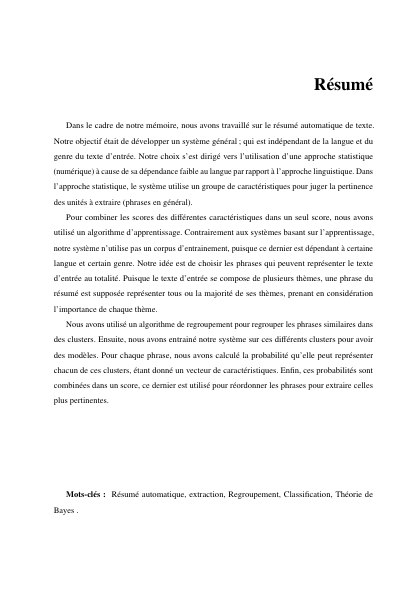
\includegraphics[width=\textwidth]{..//img/Bweb03-redaction/resume.png}
\end{minipage}

\end{frame}

\begin{frame}
\frametitle{Structure d'un rapport: Pages préliminaires}
\framesubtitle{Table des matières}

\begin{minipage}{0.52\textwidth}
	\begin{itemize}
		\item Aperçu de la structure du rapport
		\item Liste des divisions avec leurs numéros de pages 
		\item Il ne faut pas dépasser 3 niveaux de titres
		\item Si elle est placée en fin d'ouvrage
		\begin{itemize}
			\item Il est utile de fournir un sommaire
			\item Aperçu sur les parties et les chapitres
			\item Sans numéros de pages
		\end{itemize}
	\end{itemize}
\end{minipage}
\begin{minipage}{0.42\textwidth}
	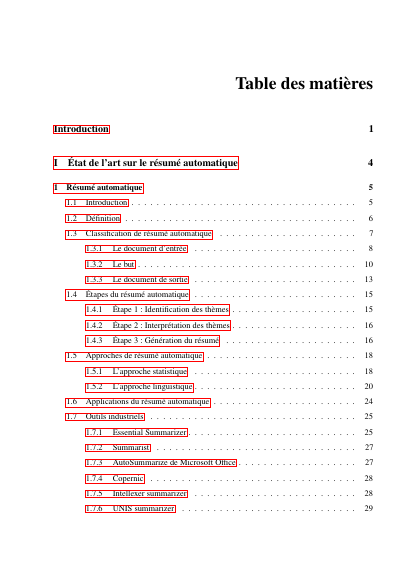
\includegraphics[width=\textwidth]{..//img/Bweb03-redaction/sommaire.png}
\end{minipage}

\end{frame}

\begin{frame}
\frametitle{Structure d'un rapport: Pages préliminaires}
\framesubtitle{Liste des illustrations (tableaux et figures)}

\begin{minipage}{0.52\textwidth}
	\begin{itemize}
		\item Une liste des tableaux et une autre pour les figures
		\item Utile pour chercher les illustrations dans le document
		\item Formée des légendes des illustrations et leurs pages
		\item La légende se forme du numéro d'apparition (soit dans le rapport entier ou dans chaque chapitre) et le titre de l'illustration.
	\end{itemize}
\end{minipage}
\begin{minipage}{0.42\textwidth}
	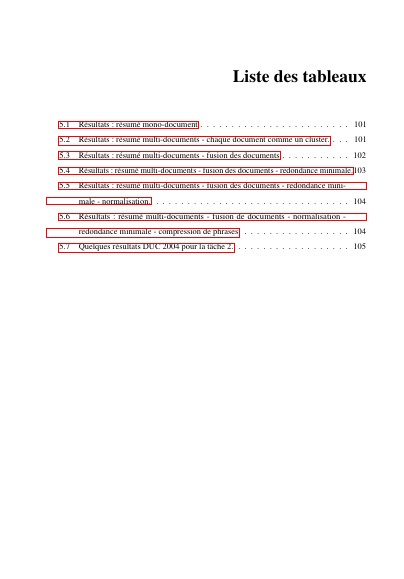
\includegraphics[width=\textwidth]{..//img/Bweb03-redaction/table-lst.png}
\end{minipage}

\end{frame}

\begin{frame}
\frametitle{Structure d'un rapport: Pages préliminaires}
\framesubtitle{Liste des abréviations}

\begin{minipage}{0.52\textwidth}
	\begin{itemize}
		\item Abréviation: forme réduite d'un mot
		\item Exemple: \expword{ESI}
		\item Facilite la lecture du document 
		\item Liste des termes et leurs définitions
		\item Ordre alphabétique des termes
	\end{itemize}
\end{minipage}
\begin{minipage}{0.42\textwidth}
	
\includegraphics[width=\textwidth]{..//img/Bweb03-redaction/abbrv-lst.png}
\end{minipage}

\end{frame}

\subsection{Corps du texte}

\begin{frame}
\frametitle{Structure d'un document}
\framesubtitle{Corps du texte}

\end{frame}

\begin{frame}
\frametitle{Structure d'un rapport: Corps du texte}
\framesubtitle{Introduction}

\begin{itemize}
	\item Contexte du travail 
	\begin{itemize}
		\item ...
		\item ...
	\end{itemize}

	\item Problématique 
	\begin{itemize}
		\item ...
		\item ...
	\end{itemize}

	\item Objectifs 
	\begin{itemize}
		\item ....
		\item ....
	\end{itemize}

	\item Plan 
	\begin{itemize}
		\item ....
		\item ....
	\end{itemize}

\end{itemize}

\end{frame}

\begin{frame}
\frametitle{Structure d'un document: Corps du texte}
\framesubtitle{Développement}

\begin{itemize}
	\item \optword{partie}: 
	\begin{itemize}
		\item regroupe des chapitres
		\item exemple: \expword{étude bibliographique}, \expword{contribution}
	\end{itemize}

	\item \optword{chapitre}:
	\begin{itemize}
		\item 
		\item 
	\end{itemize}

	\item \optword{section}: 
	\begin{itemize}
		\item section, sous-section et subdivision (3 niveaux doivent être suffisants)
		\item 
	\end{itemize}

	\item \optword{paragraphe}: 
	\begin{itemize}
		\item regroupe les phrases de la même idée
		\item 
	\end{itemize}

	\item \optword{phrase}:
	\begin{itemize}
		\item 
		\item 
	\end{itemize}
\end{itemize}

\end{frame}


\begin{frame}
\frametitle{Structure d'un document: Corps du texte}
\framesubtitle{Conclusion}

\end{frame}

\subsection{Fin du rapport}

\begin{frame}
\frametitle{Structure d'un document}
\framesubtitle{Pages complémentaires}



\end{frame}

\begin{frame}
\frametitle{Structure d'un rapport: Pages complémentaires}
\framesubtitle{Annexe a Appendice}

\begin{minipage}{0.52\textwidth}
	\begin{itemize}
		\item 
	\end{itemize}
\end{minipage}
\begin{minipage}{0.42\textwidth}
	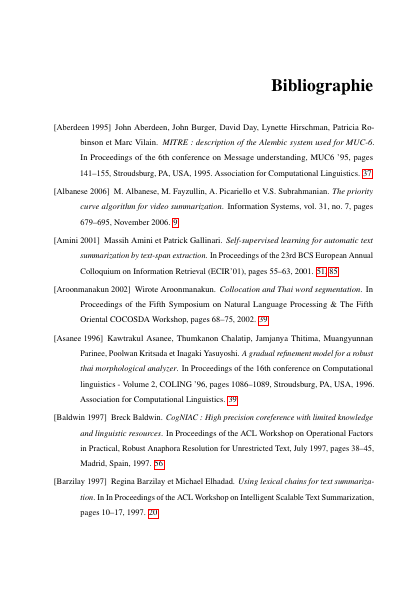
\includegraphics[width=\textwidth]{..//img/Bweb03-redaction/bibliographie.png}
\end{minipage}

\end{frame}

\begin{frame}
\frametitle{Structure d'un rapport: Pages complémentaires}
\framesubtitle{Glossaire}

\begin{minipage}{0.52\textwidth}
	\begin{itemize}
		\item 
	\end{itemize}
\end{minipage}
\begin{minipage}{0.42\textwidth}
	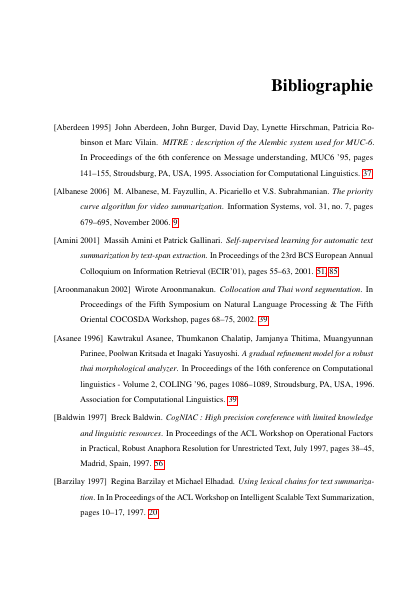
\includegraphics[width=\textwidth]{..//img/Bweb03-redaction/bibliographie.png}
\end{minipage}

\end{frame}

\begin{frame}
\frametitle{Structure d'un rapport: Pages complémentaires}
\framesubtitle{Index}

\begin{minipage}{0.52\textwidth}
	\begin{itemize}
		\item Aider le lecteur à trouver des mots ou des expressions importantes dans le document
		\item les mots communs, les noms propres, les mots clés, etc. 
		\item par exemple: les mots clés d'un langage de programmation 
		\item Si on veut indexer un mot qui n'existe pas dans le document mais qui a un mot relative, on utilise une référence croisée (renvoi) 
		\item exemple \expword{writeln ...... \itshape voir write}
	\end{itemize}
\end{minipage}
\begin{minipage}{0.42\textwidth}
	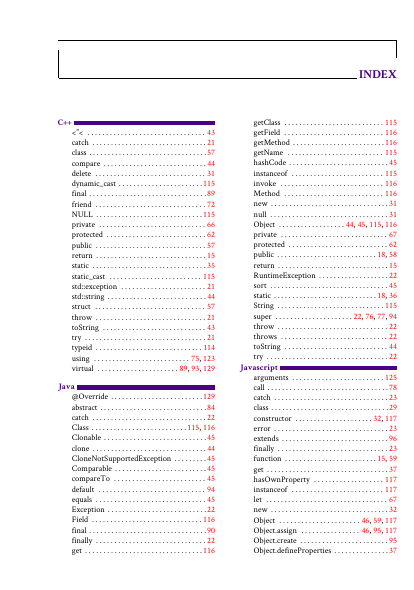
\includegraphics[width=\textwidth]{..//img/Bweb03-redaction/index.png}
\end{minipage}

\end{frame}


\begin{frame}
\frametitle{Structure d'un rapport: Pages complémentaires}
\framesubtitle{Bibliographie}

\begin{minipage}{0.52\textwidth}
	\begin{itemize}
		\item permettre au lecteur de se documenter sur les travaux antérieurs
	\end{itemize}
\end{minipage}
\begin{minipage}{0.42\textwidth}
	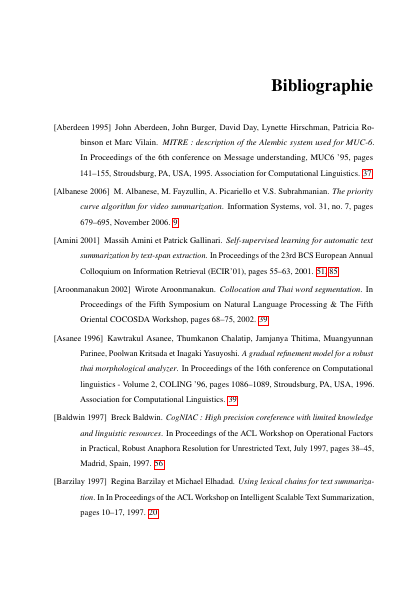
\includegraphics[width=\textwidth]{..//img/Bweb03-redaction/bibliographie.png}
\end{minipage}

\end{frame}

\begin{frame}
\frametitle{Structure d'un rapport}
\framesubtitle{Un peu d'humeur}

\vgraphpage{structure-humour.png}

\end{frame}


%===================================================================================
\section{Outils de rédaction}
%===================================================================================

\begin{frame}
\frametitle{Outils de rédaction}


\end{frame}

\subsection{Logiciels de traitement de texte}

\begin{frame}
\frametitle{Outils de rédaction}
\framesubtitle{Logiciels de traitement de texte}


\def\arraystretch{.5}

\begin{tabular}{p{.3\textwidth}cp{.5\textwidth}}%p{.3\textwidth}
	
	\hline
	
	\graphintable{.8cm}{freeoffice-logo.png} &
	\graphintable{.8cm}{freeoffice-textmaker-logo.png} &
	FreeOffice TextMaker  
	
	\url{https://www.freeoffice.com/}  \\
	\hline
	
	\graphintable{.8cm}{libreoffice-logo.png} &
	\graphintable{.8cm}{libreoffice-writer-logo.png} & 
	LibreOffice Writer 
	
	\url{https://www.libreoffice.org/}  \\
	\hline
	
	\graphintable{.8cm}{msoffice-logo.png} &
	\graphintable{.8cm}{msoffice-word-logo.png} & 
	Microsoft office Word 
	
	\url{https://www.office.com/}  \\
	\hline
	
	\graphintable{.7cm}{onlyoffice-logo.png} & &
%	\graphintable{.8cm}{onlyoffice-documents-logo.png} & 
	OnlyOffice Documents 
	
	\url{https://www.onlyoffice.com/}  \\
	\hline
	
	\graphintable{.8cm}{wps-logo.png} & 
	\graphintable{.8cm}{wps-writer-logo.png} & 
	WPS Writer
	
	\url{https://www.wps.com/}  \\
	\hline
	
	
\end{tabular}
 
\end{frame}

\subsection{\LaTeX}

\begin{frame}
\frametitle{Outils de rédaction}
\framesubtitle{\LaTeX}

\def\arraystretch{.5}

Des distributions \LaTeX :

\begin{tabular}{p{.1\textwidth}cp{.7\textwidth}}%p{.3\textwidth}
	
	\hline
	
	\graphintable{.8cm}{texlive-logo.png} &
	&
	TexLive  
	
	\url{https://www.tug.org/texlive/}
	
	Ubuntu: \expword{apt install texlive-full}\\
	\hline
	
	\graphintable{.8cm}{miktex-logo.png} &
	& 
	MiKTex 
	
	\url{https://miktex.org/download}  \\
	\hline
	
\end{tabular}

\vspace{\fill}

Des éditeurs \LaTeX :

\begin{tabular}{p{.1\textwidth}cp{.7\textwidth}}%p{.3\textwidth}
	
	\hline
	
	\graphintable{.8cm}{texstudio-logo.png} &
	&
	TexStudio  
	
	\url{http://www.texstudio.org/}  \\
	\hline
	
	\graphintable{.8cm}{lyx-logo.png} &
	& 
	LyX (WYSIWYM)
	
	\url{https://www.lyx.org/}  \\
	\hline
	
\end{tabular}

\end{frame}


\subsection{Rédaction en ligne}


\begin{frame}
\frametitle{Outils de rédaction}
\framesubtitle{Rédaction en ligne}

\def\arraystretch{.5}

\begin{tabular}{p{.1\textwidth}cp{.7\textwidth}}%p{.3\textwidth}
	
	\hline
	
	\graphintable{.8cm}{google-docs-logo.png} &
	&
	Google Docs  
	
	\url{http://docs.google.com/document/}  \\
	\hline
	
	\graphintable{.8cm}{msoffice-word-logo.png} &
	&
	Microsoft Office Word 
	
	\url{https://www.office.com/launch/word}  \\
	\hline
	
	\graphintable{.8cm}{icloud-pages-logo.png} &
	&
	iCloud Pages 
	
	\url{https://www.icloud.com/pages/}  \\
	\hline
	
	\graphintable{.8cm}{overleaf-logo.png} &
	&
	Overleaf (\LaTeX) 
	
	\url{https://www.overleaf.com/}  \\
	\hline
	
\end{tabular}

\end{frame}

\begin{frame}
\frametitle{Outils de rédaction: Rédaction en ligne}
\framesubtitle{Google Docs Document}

\vgraphpage{google-docs-preview.png}

\end{frame}

\begin{frame}
\frametitle{Outils de rédaction: Rédaction en ligne}
\framesubtitle{Microsoft Office Word}

\vgraphpage{msoffice-word-preview.png}

\end{frame}

\begin{frame}
\frametitle{Outils de rédaction: Rédaction en ligne}
\framesubtitle{iCloud Pages}

\vgraphpage{icloud-pages-preview.png}

\end{frame}

\begin{frame}
\frametitle{Outils de rédaction: Rédaction en ligne}
\framesubtitle{Overleaf}

\vgraphpage{overleaf-preview.png}

\end{frame}

\begin{frame}
\frametitle{Outils de rédaction}
\framesubtitle{Un peu d'humeur}

\vgraphpage{tools-humour.png}

\end{frame}

\nocite{*}
%\subsection{Bibliography}
%\frame[allowframebreaks]%
%{\frametitle{Références}
%\tiny
%\bibliography{Bweb01}
%\bibliographystyle{plain} 
%}

\begin{multicols*}{2}[\usebeamertemplate*{frametitle}\frametitle{Références}]%
	\tiny
	\bibliography{Bweb03}
	\bibliographystyle{acm}
\end{multicols*}


\end{document}

